\documentclass[a4paper,12pt]{article}
\usepackage{amsmath, amssymb, graphicx}
\usepackage{hyperref}
\usepackage{geometry}
\usepackage{subfiles}
\usepackage{tikz}
\usepackage{framed}
\usepackage{stmaryrd} 
\usepackage{listings}
\usepackage{booktabs}
\usepackage{printlen, printsudoku}
\usepackage{subcaption}  % for subfigures
\usepackage{caption}  
\usepackage{algorithm}
\usepackage{algorithmic}
\geometry{margin=1in}
\newcommand{\mean}[1]{\{\!\!\{#1\}\!\!\}} 
\title{Numerical Solution of the Porous Medium Equation using the LDG Method}
\author{Nikolaus Vohwinkel}
\date{\today}


\newcommand\restr[2]{{% we make the whole thing an ordinary symbol
		\left.\kern-\nulldelimiterspace % automatically resize the bar with \right
		#1 % the function
		\littletaller % pretend it's a little taller at normal size
		\right|_{#2} % this is the delimiter
}}

\begin{document}
	\maketitle
	
	\begin{abstract}
	The porous medium equation (PME) is a nonlinear partial differential equation that models diffusion in porous media. In this Forschungsmodul, the Local Discontinuous Galerkin (LDG) method is employed to numerically solve the PME. The well-established method is tested in various settings, using different polynomial orders of basis functions, to study their effects on the solution’s behavior. Furthermore, a hyperbolic system that degenerates into the PME under certain parameter regimes is investigated. For both approaches, extensive numerical results are presented to illustrate the capabilities and limitations of each method.
	\end{abstract}
	
	\section{Introduction}
The porous medium equation (PME) without source and advection terms is given by:
\[
\frac{\partial u}{\partial t} = \Delta (u^m), \quad x \in \Omega, \quad t > 0,
\]
where \( m > 1 \) is a constant characterizing the medium's porosity. This equation models various physical processes, including gas flow in porous media and heat transfer in plasmas, where \( u \) typically represents a concentration or temperature that must remain nonnegative for all times. Assuming that the initial condition \( u_0 \) is nonnegative, the PME can be rewritten as:
\[
\frac{\partial u}{\partial t} = \Delta (u^m) = \nabla \cdot (m u^{m-1} \nabla u) = \nabla \cdot (a(u)\nabla u), \quad x \in \Omega, \quad t > 0,
\]
where \( a(u) = m u^{m-1} \geq 0 \). Thus, the PME can be identified as a nonlinear diffusion equation of the degenerate parabolic type, since it degenerates when \( u=0 \). Notably, if the initial data has compact support, the solution of the initial value problem for the PME will also have compact support at any given time \( t>0 \). Due to this feature, the PME exhibits finite speed of propagation at the moving front or ``free boundary'' region where the solution vanishes. Another interesting property of the PME is the so-called waiting time phenomenon, which can occur for specially chosen initial data. In this case, the free boundary remains stationary until a finite positive time (the waiting time), after which it instantaneously moves with finite speed.\\
A fundamental example of a solution is the Barenblatt (or source-type) solution \cite{Barenblatt}, which can be written explicitly as:
\begin{equation}
	\label{eq:barenblatt function}
	B_m(x, t)=t^{-k}\left[\left(1-\frac{k(m-1)}{2 m} \frac{|x|^2}{t^{2 k}}\right)_{+}\right]^{1 /(m-1)},
\end{equation}
where \( (u)_{+}=\max (u, 0) \) and \( k=1/(m+1) \). For any time \( t>0 \), this solution has compact support \(\left[-\alpha_m(t), \alpha_m(t)\right]\), with the interface \(|x|=\alpha_m(t)\) moving outward at finite speed, where
\[
\alpha_m(t)=\sqrt{\frac{2 m}{k(m-1)}} \cdot t^k.
\]
This solution will later be useful for assessing the accuracy of the numerical methods presented. In this work, two numerical frameworks will be tested. One relies on the Local Discontinuous Galerkin (LDG) formulation proposed by Zhang and Wu \cite{Zhang2009}, while the other employs a hyperbolic system that degenerates into the PME as the parameter \(\varepsilon \to 0\), similar to the system introduced by Jin, Pareschi, and Toscani \cite{Jin1998}. Both approaches utilize a Galerkin ansatz on discontinuous basis functions of varying polynomial degree. Since this ansatz tends to produce oscillations near the free boundary, the LDG method addresses this issue by introducing an artificial diffusion parameter \(\gamma\) and employing limiters extensively in the vicinity of the free boundary. However, for the hyperbolic system, these oscillations are unavoidable, as will be demonstrated by the findings in this work. 


%-------------------------------------------------------------------------------------------------------%
\section{Mathematical and numerical Formulation}
To approximate solutions of the porous medium equation (PME), we discretize the spatial domain using a finite number of non-overlapping cells and apply a high-order accurate numerical method tailored for problems with nonlinear diffusion and potential degeneracies. Specifically, we employ the Discontinuous Galerkin (DG) method, known for its flexibility in handling complex boundary conditions, its ability to use high-order polynomial approximations, and its local conservation properties.\\
\\
The computational domain is divided into \( N_{\text{cells}} \in \mathbb{N} \) cells, where each cell
\[
I_i = \left(x_{i-\frac{1}{2}}, x_{i+\frac{1}{2}}\right)
\]
has width 
\[
h_i = x_{i+\frac{1}{2}} - x_{i-\frac{1}{2}}, \quad i = 1, \ldots, N_{\text{cells}}.
\]
Since we use the DG approach in both schemes, we adopt an ansatz that separates spatial and temporal dependencies of the solution. Within each cell \( I_i \), the approximate solutions are represented as
\[
u_h(x,t)\big|_{I_i} = \sum_{l=0}^n u_i^l(t)\,\varphi_h^l(x), \quad
j_h(x,t)\big|_{I_i} = \sum_{l=0}^n j_i^l(t)\,\varphi_h^l(x), \quad
q_h(x,t)\big|_{I_i} = \sum_{l=0}^n q_i^l(t)\,\varphi_h^l(x),
\]
where the basis functions \(\varphi_h^l\) are scaled Legendre polynomials defined by
\[
\varphi_h^l(x) = p_l\left(\frac{x - x_i}{h_i}\right), \quad x \in I_i,
\]
and \( p_l \) denotes the Legendre polynomial of degree \( l \in \mathbb{N}_0 \).
For the initial solution \( u_h(0) \), we use the \( L^2 \)-projection of the given initial data \( u_0 \) into the discrete function space
\[
V_h^n = \left\{ v_h : \mathbb{R} \to \mathbb{R} \;\middle|\; v_h|_{I_i} \in \mathcal{P}_n(I_i), \forall i=1,\ldots,N_{\text{cells}} \right\},
\]
where \( \mathcal{P}_n(I_i) \) denotes the space of polynomials of degree at most \( n \) on the cell \( I_i \). The initial projection satisfies
\[
\int_{I_i} \left(u_h(0,x) - u_0(x)\right) \varphi_h(x) \, dx = 0, \quad \forall \varphi_h \in V_h^n, \quad \forall i=1,\ldots,N_{\text{cells}}.
\]
The Legendre polynomials and their derivatives are computed using\\ Algorithm 22: \texttt{LegendrePolynomialAndDerivative} from Kopriva \cite{Kopriva2009}. To accurately evaluate integrals, we employ Gauss–Legendre quadrature with nodes and weights obtained from Algorithm 23: \texttt{LegendreGaussNodesAndWeights} (also from Kopriva), allowing for flexible polynomial degrees.

\begin{figure}[h]
	\centering
	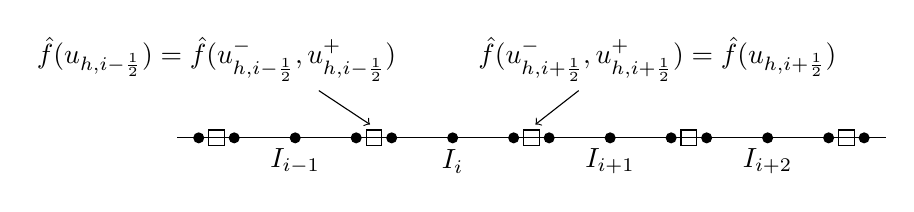
\begin{tikzpicture}
		\draw (2.5,0) -- (11.5,0);
		\foreach \x in {2.774597, 3.225403, 4, 4.774597, 5.225403, 6, 6.774597, 7.225403, 8, 8.774597, 9.225403, 10, 10.774597, 11.225403} {
			\fill (\x,0) circle (2pt);
		}
		\foreach \x in {3, 5, 7, 9, 11} {
			\draw (\x-0.1,-0.1) rectangle (\x+0.1,0.1);
		}
		\node at (4,-0.3) {\(I_{i-1}\)};
		\node at (6,-0.3) {\(I_i\)};
		\node at (8,-0.3) {\(I_{i+1}\)};
		\node at (10,-0.3) {\(I_{i+2}\)};
		\node at (3,1) {\(\hat{f}(u_{h,i-\frac{1}{2}}) = \hat{f}(u_{h,i-\frac{1}{2}}^-, u_{h,i-\frac{1}{2}}^+)\)};
		\draw[<-] (4.95,.17) -- (4.3,0.6);
		\node at (8.6,1) {\(\hat{f}(u_{h,i+\frac{1}{2}}^-, u_{h,i+\frac{1}{2}}^+) = \hat{f}(u_{h,i+\frac{1}{2}})\)};
		\draw[<-] (7.05,.17) -- (7.6,0.6);
	\end{tikzpicture}
	\caption{Example cells with Gauss nodes and interface fluxes for polynomial degree \( n=3 \).}
	\label{fig:example_cells}
\end{figure}


%-------------------------------------------------------------------------------------------------------------%

\subsection{The Local Discontinuous Galerkin (LDG) Method}
A common strategy for addressing the nonlinearity in the porous medium equation (PME) is to introduce auxiliary variables, which facilitate the construction of a Local Discontinuous Galerkin (LDG) scheme. By carefully selecting appropriate numerical fluxes at element interfaces, the resulting formulation can be shown to be \( L^2 \)-stable.To apply the LDG method, we first rewrite the PME in first-order form by introducing auxiliary variables \( g \) and \( q \):
\begin{align*}
	\partial_t u + \partial_x\left[f(u) - \sqrt{a(u)}\,q\right] &= s(u), \quad x \in I,~t > 0, \\
	q - \partial_x g &= 0, \quad x \in I,~t > 0,
\end{align*}
where
\[
g(u) = \int_0^u \sqrt{a(s)}\,ds, \quad \text{with} \quad a(u) = m u^{m-1}.
\]
Following the LDG approach Zhang and Wu \cite{Zhang2009} therefore defined numerical fluxes to handle discontinuities at element interfaces. The semi-discrete formulation in a cell \( I_i \) becomes:
\begin{equation}
	\label{eq:ldg}
	\begin{aligned}
		\partial_t u_i^l(t) &= \frac{2l+1}{h} \int_{I_i} \left[ s(u_h) \varphi^l(x) + \left( f(u_h) - \sqrt{a(u_h)}\,q_h \right) \partial_x \varphi^l(x) \right]\,dx \\
		&\quad - \frac{2l+1}{h} \left[ \left( \hat{f}(u_h) - \frac{\llbracket g(u_h) \rrbracket}{\llbracket u_h \rrbracket} \mean{q_h} - \gamma \llbracket q_h \rrbracket \right) \varphi^l(x) \right]_{x_{i-\frac{1}{2}}}^{x_{i+\frac{1}{2}}}, \\
		q_i^l(t) &= -\frac{2l+1}{h} \int_{I_i} g(u_h) \partial_x \varphi^l(x)\,dx + \left[ \left( -\mean{g(u_h)} + \gamma \llbracket u_h \rrbracket \right) \varphi^l(x) \right]_{x_{i-\frac{1}{2}}}^{x_{i+\frac{1}{2}}},
	\end{aligned}
\end{equation}
where \( \mean{\cdot} \) and \( \llbracket \cdot \rrbracket \) denote the arithmetic mean and jump operators, respectively, defined at cell interfaces as:
\[
\mean{g(u_h)} = \frac{g(u_h^+) + g(u_h^-)}{2}, \quad
\llbracket u_h \rrbracket = u_h^+ - u_h^-.
\]
When \( \llbracket u_h \rrbracket \neq 0 \), the term
\[
\frac{\llbracket g(u_h) \rrbracket}{\llbracket u_h \rrbracket}
\]
is well-defined and serves as an approximation of \( \sqrt{a(u_h)} \). However, when \( \llbracket u_h \rrbracket = 0 \), this expression becomes undefined. To preserve numerical stability and ensure a meaningful evaluation in such cases, it is customary to replace the undefined ratio with
\[
\sqrt{a(u_h)}.
\]
The numerical behavior of this replacement critically depends on how equality is determined between \( u_h^+ \) and \( u_h^- \). A very strict tolerance, such as that dictated by \textit{long double} precision (approximately \(10^{-18}\) to \(10^{-19}\)) can result in undesirable or unstable behavior. Therefore, we adopt the adaptive tolerance criterion recommended by Kopriva~\cite{Kopriva2009} (Algorithm 139: \texttt{AlmostEqual}), which ensures a more robust and stable scheme by using a practical threshold for comparing floating-point values.

%------------------------------------------------------------------------------------------------------------%
\subsection{Hyperbolic balance law}
Another approach to approximate the porous medium equation is to consider a hyperbolic system that degenerates to the porous medium equation as \( \varepsilon \to 0 \), similar to the method proposed by Jin, Pareschi, and Toscani in \cite{Jin1998}. 
To this end, we introduce an auxiliary variable \( \mathbf{j} \) and a relaxation parameter \( \varepsilon \), leading to the following hyperbolic balance law:
\begin{equation}
	\begin{aligned}
		\partial_t u^{\varepsilon} + \nabla \cdot \mathbf{j}^{\varepsilon} &= 0, \\
		\varepsilon \partial_t \mathbf{j}^{\varepsilon} + \nabla \left( \left( u^{\varepsilon} \right)^m \right) &= -\mathbf{j}^{\varepsilon}.
	\end{aligned}
\end{equation}
For spatial discretization, we employ the Discontinuous Galerkin (DG) method using Legendre polynomials as basis functions. This yields the following semi-discrete formulation over a cell \( I_i \):
\begin{equation}
	\begin{aligned}
		\int_{I_i} \partial_t \left( \sum_{l=0}^{n} u_i^l(t) \varphi^l(x) \right) \varphi^r(x) \, dx 
		&+ \int_{I_i} \partial_x \left( \sum_{l=0}^{n} j_i^l(t) \varphi^l(x) \right) \varphi^r(x) \, dx = 0, \\
		\int_{I_i} \varepsilon \, \partial_t \left( \sum_{l=0}^{n} j_i^l(t) \varphi^l(x) \right) \varphi^r(x) \, dx 
		&+ \int_{I_i} \partial_x (u_h^m) \, \varphi^r(x) \, dx = -\int_{I_i} j_h \, \varphi^r(x) \, dx.
	\end{aligned}
\end{equation}
Projecting onto the Legendre basis and exploiting orthogonality, we obtain the following system of ODEs for the modal coefficients \( u_i^l(t) \) and \( j_i^l(t) \):
\begin{equation}
	\begin{aligned}
		\partial_t u_i^l(t) &= \frac{2l+1}{h_i} \int_{I_i} j_h \left( \varphi_h^l \right)_x \, dx 
		- \frac{2l+1}{h_i} \left[ \widehat{j}_h \varphi_h^l \right]_{x_{i-\frac{1}{2}}}^{x_{i+\frac{1}{2}}}, \\
		\varepsilon \, \partial_t j_i^l(t) &= -\frac{2l+1}{h_i} \int_{I_i} j_h \, \varphi_h^l \, dx 
		+ \frac{2l+1}{h_i} \int_{I_i} (u_h)^m \left( \varphi_h^l \right)_x \, dx 
		- \frac{2l+1}{h_i} \left[ \widehat{u}_h \varphi_h^l \right]_{x_{i-\frac{1}{2}}}^{x_{i+\frac{1}{2}}},
	\end{aligned}
\end{equation}
where \( \widehat{j}_h \) and \( \widehat{u}_h \) are appropriate numerical fluxes defined at the cell interfaces to ensure stability and consistency.

%-------------------------------------------------------------------------------------------------------------%

\subsection{Limiter}
In order to obtain accurate and stable simulations, two limiters are introduced, both of which utilize a first-order $L^2$-projection of $u_h$. To implement this projection, we employ a least-squares approach that remains as close as possible to the original numerical solution, thereby ensuring that the projection remains approximately mass-conserving.
\subsubsection{First-Order Slope Limiter}
The general formulation of the first-order slope-limited approximation is given by
\begin{equation*}
	u_h|_{I_i} = \bar{u}_i + (x - x_i) u_{x,i}, \quad i = 1, 2, \ldots, N_{\text{cells}},
\end{equation*}
where $u_{x,i}$ is the slope, and $\bar{u}_i$ is the average solution in cell $I_i$. The slope is limited using the modified minmod function:
\begin{equation*}
	\Lambda \Pi^1_h u_h |_{I_i} = \bar{u}_i + (x - x_i) \bar{m} \left( u_{x,i}, \frac{\bar{u}_i - \bar{u}_{i-1}}{h_i/2}, \frac{\bar{u}_{i+1} - \bar{u}_i}{h_i/2} \right),
\end{equation*}
where
\begin{equation*}
	\bar{m}(a_1, a_2, a_3) = 
	\begin{cases}
		a_1, & \text{if } |a_1| \leq \mu h^2, \\
		s \min(|a_1|, |a_2|, |a_3|), & \text{if } |a_1| > \mu h^2 \text{ and } s = \operatorname{sgn}(a_k),\ k = 1,2,3, \\
		0, & \text{otherwise}.
	\end{cases}
\end{equation*}
The limiter is applied in such a way that it preserves the current boundary values of the solution unless their deviation from the cell average is too large. This enforcement is given by:
\begin{equation*}
	\begin{aligned}
		\Lambda \Pi^1_h u_{h, i+1/2}^{-} &= \bar{u}_i + \bar{m}(u_{i+1/2}^{-} - \bar{u}_i, \bar{u}_i - \bar{u}_{i-1}, \bar{u}_{i+1} - \bar{u}_i), \\
		\Lambda \Pi^1_h u_{h, i-1/2}^{+} &= \bar{u}_i - \bar{m}(\bar{u}_i - u_{i-1/2}^{+}, \bar{u}_i - \bar{u}_{i-1}, \bar{u}_{i+1} - \bar{u}_i).
	\end{aligned}
\end{equation*}
If the following conditions hold:
\[
\Lambda \Pi^1_h u_{h, i+1/2}^{-} = u_{i+1/2}^{-} \quad \text{and} \quad \Lambda \Pi^1_h u_{h, i-1/2}^{+} = u_{i-1/2}^{+},
\]
then no limiting is needed. Otherwise, a local first-order $L^2$-projection $u_h^1$ of $u_h$ is computed, and the limiter $\Lambda \Pi^1$ is reapplied.

\subsubsection{Second Limiter: Positivity Preservation}

The slope limiter alone does not guarantee non-negativity within the cell, which is essential due to the presence of square roots in the model. To enforce positivity, a second limiting step is introduced:

\begin{enumerate}
	\item If any value in a cell is negative, compute a local first-order $L^2$-projection $u_h^1$ of $u_h$.
	\item Calculate the average value $\bar{u}_i$ and apply the second limiter $P\Pi u_h^1$.
\end{enumerate}
This second limiter reconstructs a linear function based on the cell average to ensure positivity throughout the cell:
\begin{equation*}
	P \Pi^1_h u_h^1 = 
	\begin{cases}
		\left[1 - \frac{2(x - x_i)}{h_i} \right] \bar{u}_i, & \text{if } u_{h, i+1/2}^{-} < 0, \\
		\left[1 + \frac{2(x - x_i)}{h_i} \right] \bar{u}_i, & \text{if } u_{h, i-1/2}^{+} < 0.
	\end{cases}
\end{equation*}
This reconstruction ensures that the solution is bounded, continuous, and positive throughout the cell. The general $L^2$-projected linear function takes the form:
\begin{equation*}
	f(x) = \left( u_{i+1/2}^{-} - u_{i-1/2}^{+} \right) \frac{x - x_i}{h_i} + \frac{1}{2} \left( u_{i+1/2}^{-} + u_{i-1/2}^{+} \right).
\end{equation*}
Assuming only one interface value is negative, we modify the solution such that:
\[
\bar{u}_i = \frac{1}{2} \left( u_{i+1/2}^{-} + u_{i-1/2}^{+} \right),
\]
which preserves the cell average and ensures:
\[
2|\bar{u}_i| < u_{i-1/2}^{+} \quad \text{or} \quad 2|\bar{u}_i| < u_{i+1/2}^{-}.
\]
This ensures that the reconstruction does not introduce new extrema. Since the negative interface value is clamped to zero, the total variation does not increase, thus maintaining the TVD (total variation diminishing) property.
\paragraph{Handling Negative Cell Averages}
While Zhang and Wu \cite{Zhang2009} showed that their method avoids negative cell averages for polynomial degree $l = 0$, the numerical experiments provided in this work indicate this does not always hold in practice for varying polynomial degrees. Therefore, as a final safeguard:
\begin{equation*}
	P \Pi^1_h u_h^1 = 
	\begin{cases}
		\left[1 - \frac{2(x - x_i)}{h_i} \right] \bar{u}_i, & \text{if } u_{h, i+1/2}^{-} < 0, \\
		\left[1 + \frac{2(x - x_i)}{h_i} \right] \bar{u}_i, & \text{if } u_{h, i-1/2}^{+} < 0, \\
		0, & \text{if } \bar{u}_i < 0,
	\end{cases}
\end{equation*}
is used to avoid such cases.
%-------------------------------------------------------------------------------------------------------------%
\subsection{Time-stepping}
%-------------------------------------------------------------------------------------------------------------%
For time discretization of the semi-discrete Discontinuous Galerkin (DG) formulation, we employ a third-order explicit Runge-Kutta scheme. The system can be written as
\[
\frac{\mathrm{d} u_h}{\mathrm{d} t} = \mathbb{M}^{-1} \operatorname{RHS}(u_h) = \mathcal{L}_h(u_h), \quad t \in (0, T),
\]
where \(\mathbb{M}\) is the mass matrix and \(\operatorname{RHS}(u_h)\) represents the spatial DG discretization operator.
The third-order Runge-Kutta update from time \( t^n \) to \( t^{n+1} = t^n + \Delta t^n \) is given by:
\[
\begin{aligned}
	u^{(1)} &= u_h^n + \Delta t^n \, \mathcal{L}_h\big(u_h^n\big), \\
	u^{(2)} &= \frac{3}{4} u_h^n + \frac{1}{4} u^{(1)} + \frac{1}{4} \Delta t^n \, \mathcal{L}_h\big(u^{(1)}\big), \\
	u_h^{n+1} &= \frac{1}{3} u_h^n + \frac{2}{3} u^{(2)} + \frac{2}{3} \Delta t^n \, \mathcal{L}_h\big(u^{(2)}\big).
\end{aligned}
\]
The time step \(\Delta t^n\) must satisfy appropriate stability restrictions. These are given for the two considered schemes by:
\begin{align}
	\text{LDG:} \quad
	\frac{\max |f'(u_h^n)| \, \Delta t^n}{\Delta x} + \frac{2 \max |a(u_h^n)| \, \Delta t^n}{(\Delta x)^2} &\leq\textit{CFL}  \cdot \frac{1}{PP_N + 1}, \\
	\text{Hyperbolic relaxation:} \quad
	\frac{\max |u_h^n| \, \Delta t^n}{\Delta x \sqrt{\varepsilon}} + \frac{2 \max |j_h^n| \, \Delta t^n}{(\Delta x)^2 \varepsilon} &\leq \textit{CFL} \cdot \frac{1}{PP_N + 1},
\end{align}
where \(PP_N\) denotes the polynomial degree plus one (the number of basis functions per cell), and \textit{CFL} is the Courant–Friedrichs–Lewy number chosen based on stability considerations. For example, Zhang and Wu \cite{Zhang2009} have chosen the \textit{CFL} number as \( \mathrm{\textit{CFL}} = 0.02 \) when using a polynomial degree of \( l = 2 \).
%-------------------------------------------------------------------------------------------------------------%
%-------------------------------------------------------------------------------------------------------------%
\clearpage
\section{Practical Implementation}
For the implementation, \texttt{C++} was used along with the standard \texttt{vector} and \texttt{cmath} libraries for numerical operations, and the \texttt{VTK} library to generate output data. All calculations were performed in double precision. However, for fine grids and high polynomial degrees, higher-precision floating-point arithmetic may be required, as values near kinks can become extremely small and diffuse across the grid, which may not be adequately captured by standard double precision. Additionally, for polynomial degrees \( l > 15 \), a more accurate algorithm for computing Gauss–Legendre nodes must be employed.
\\

\begin{figure}[htbp]
	\centering
	\fbox{
		\resizebox{0.5\textwidth}{!}{%
			\begin{minipage}{\textwidth}
				\begin{framed}
					\noindent
					\textbf{Output Name:} \texttt{BBM2N160PP5}
					
					\noindent
					\textbf{Polynomial Degree:} $P=5$
					
					\noindent
					\textbf{Physical Domain:} \\
					$\quad$ Start: $-5$ \\
					$\quad$ End: $5$
					
					\noindent
					\textbf{End Time:} $1.0$
					
					\noindent
					\textbf{Numerical Parameters:} \\
					$\quad$ Flux Function: \texttt{barenblatt} \\
					$\quad$ Riemann Solver: \texttt{upwind} \\
					$\quad$ Epsilon: $0.0$
					
					\noindent
					\textbf{Limiter Parameters:} \\
					$\quad$ Use Limiter: \texttt{true} \\
					$\quad$ Use Modified Limiter: \texttt{true} 
					
					\noindent
					\textbf{Time Stepping:} \\
					$\quad$ CFL: $0.002$ \\
					$\quad$ Scheme: \texttt{RK} (Runge-Kutta) \\
					$\quad$ Maximum $\Delta t$: $1\times10^{-6}$
					
					\noindent
					\textbf{Output:} \\
					$\quad$ Write State Frequency: $10000$
					
					\noindent
					\textbf{Initial Condition:} \\
					$\quad$ Type: \texttt{barenblatt} 
					
					\noindent
					\textbf{Barenblatt Parameters:} \\
					$\quad$ $M=2$ \\
					$\quad$ Time: $1.0$\\
					$\quad$ Use Source: \texttt{true} \\
					$\quad$ Use Transport: \texttt{false} \\
					$\quad$ Transport Flux: \texttt{linear}
					
					\noindent
					\textbf{Error Parameters:} \\
					$\quad$ Error interval A: $-1.5$ \\
					$\quad$ Error interval B: $1.5$
					
					\noindent
					\textbf{Discretization:} \\
					$\quad$ Number of Cells: $160$
				\end{framed}
			\end{minipage}
		}
	}
	\caption{Example parameter.ini file.}
\end{figure}

\begin{algorithm}
	\caption{Example algorithm with loops and initialization}
	\begin{algorithmic}[1]
		\STATE \textbf{Input:} $N_{cells}$, $m$, $PP_N$, $u_0$, \textit{flux, useSource, useTransport, numFlux, CFL}, $\varepsilon$,
		\STATE \textbf{Initialize:}
		\STATE $\quad u \gets 0$ \COMMENT{Solution array}
		\STATE $\quad dx \gets \frac{1}{N_x - 1}$ \COMMENT{Grid spacing}
		\STATE $\quad dy \gets \frac{1}{N_y - 1}$
		
		\FOR{$i=1$ to $N_x$}
		\FOR{$j=1$ to $N_y$}
		\STATE $x \gets (i - 1) \cdot dx$
		\STATE $y \gets (j - 1) \cdot dy$
		\STATE $u(i, j) \gets \text{initial condition at } (x, y)$
		\ENDFOR
		\ENDFOR
		
		\STATE \textbf{Output:} Solution array $u$
	\end{algorithmic}
\end{algorithm}
%=============================================================================================================%
\clearpage
\section{Numerical Results}
All numerical simulations were performed on an Intel i7-3600K processor equipped with 16\,GB of DDR3 RAM. The computational domain was \([-6,6]\), and unless stated otherwise, all error calculations were conducted on the subdomain \([-1.5,1.5]\).
\paragraph{Local Discontinuous Galerkin}  
To initiate the simulation, one must select the artificial diffusion parameter \(\gamma\). Zhang and Shu~\cite{Zhang2009} proposed the following formulation:
\[
\gamma_{j+\frac{1}{2}} =
\begin{cases}
	\frac{1}{2} \dfrac{g_{j+1} - g_j}{u_{j+1} - u_j}, & \text{if } u_{j+1} \neq u_j, \\[10pt]
	\frac{1}{2} \sqrt{a(u_{h,j})}, & \text{otherwise}.
\end{cases}
\]
This approach has been analytically justified and is suggested to extend naturally to higher-order polynomial basis functions beyond the case of polynomial degree \(l=0\).
In the following numerical experiments, no stability issues were encountered, even for high exponents such as \(m=8\), when the Barenblatt solution~(\ref{eq:barenblatt function}) was used as the initial condition at \(t=1\,\mathrm{s}\). However, the accuracy of the numerical scheme appears to depend on the nonlinearity:
\begin{itemize}
	\item For odd exponents \(m\), the number of limiter calls is significantly reduced, and the experimental order of convergence (EOC) is maintained.
	\item In contrast, for even exponents, the number of limiter calls increases substantially, and no improvement in accuracy is observed with \(h\)-refinement.
\end{itemize}
\begin{table}[h]
	\centering
	\begin{minipage}[t]{0.49\linewidth}
		\centering
		\resizebox{\linewidth}{!}{%
			\begin{tabular}{cccccccc}
				\hline
				$N$ & $L^2$ Error & EOC$_{L^2}$ & $L^\infty$ Error & EOC$_{L^\infty}$ & \#1st Lim. & \#2nd Lim. & \#steps\\
				\hline
				10 & 4.52e-03 & - & 1.12e-02 & - & 227 & 336 & 56\\
				20 & 3.05e-03 & 0.57 & 6.30e-03 & 0.83 & 1302 & 1332 & 222\\
				40 & 3.21e-03 & -0.08 & 4.91e-03 & 0.36 & 10092 & 12868 & 883\\
				80 & 3.19e-03 & 0.01 & 3.95e-03 & 0.31 & 41119 & 42649 & 3530\\
				160 & 3.18e-03 & 0.00 & 3.50e-03 & 0.18 & 167100 & 166384 & 14115\\
				320 & 3.18e-03 & 0.00 & 3.28e-03 & 0.09 & 664708 & 1605483 & 56455\\
				\hline
			\end{tabular}
		}
		\caption{Convergence results for $P=1$, $m=8$}
		\label{table:BBM8P1}
	\end{minipage}
	\hfill
	\begin{minipage}[t]{0.49\linewidth}
		\centering
		\resizebox{\linewidth}{!}{%
			\begin{tabular}{cccccccc}
				\hline
				$N$ & $L^2$ Error & EOC$_{L^2}$ & $L^\infty$ Error & EOC$_{L^\infty}$ & \#1st Lim. & \#2nd Lim. & \#steps\\
				\hline
				10 & 2.28e-04 & - & 6.45e-04 & - & 509 & 365 & 82\\
				20 & 5.37e-05 & 2.09 & 9.30e-05 & 2.79 & 3375 & 404 & 328\\
				40 & 5.23e-05 & 0.04 & 6.80e-05 & 0.45 & 8426 & 7851 & 1309\\
				80 & 5.20e-05 & 0.01 & 5.75e-05 & 0.24 & 53905 & 23397 & 5234\\
				160 & 5.19e-05 & 0.00 & 5.37e-05 & 0.10 & 233769 & 67510 & 20935\\
				320 & 5.19e-05 & 0.00 & 5.29e-05 & 0.02 & 820520 & 393031 & 83738\\
				\hline
			\end{tabular}
		}
		\caption{Convergence results for $P=2$, $m=8$}
		\label{table:BBM8P2}
	\end{minipage}
	\vspace{0.5cm}
	\begin{minipage}[t]{0.49\linewidth}
		\centering
		\resizebox{\linewidth}{!}{%
		\begin{tabular}{cccccccc}
			\hline
			$N$ & $L^2$ Error & EOC$_{L^2}$ & $L^\infty$ Error & EOC$_{L^\infty}$ & \#1st Lim. & \#2nd Lim.& \#steps\\
			\hline
			10 & 1.40e-04 & - & 9.53e-04 & - & 1009 & 557 & 110\\
			20 & 5.26e-07 & 8.05 & 1.86e-06 & 9.00 & 3955 & 2743 & 437\\
			40 & 4.59e-07 & 0.20& 6.22e-07 & 1.58 & 20872 & 19004 & 1745\\
			80 &  4.59e-07 & 0.00 & 4.92e-07 & 0.34 & 66962 & 52520 & 6977\\
			160 & 4.59e-07 & 0.00 & 4.70e-07 & 0.07 & 327605 & 265718 & 27908\\
			320 & 4.59e-07 & 0.00 & 4.70e-07 & 0.00 & 1521531 & 339425 & 1025272\\
			\hline
		\end{tabular}}
		\caption{Convergence results for P=3, M=8}
		\label{table:BBM8P3}
	\end{minipage}
	\hfill
		\begin{minipage}[t]{0.49\linewidth}
		\centering
		\resizebox{\linewidth}{!}{%
	\begin{tabular}{cccccccc}
		\hline
		$N$ & $L^2$ Error & EOC$_{L^2}$ & $L^\infty$ Error & EOC$_{L^\infty}$ & \#1st Lim. & \#2nd Lim.& \#steps\\
		\hline
		10 & 2.61e-05 & - & 1.67e-04 & - & 1085 & 807 & 137\\
		20 & 3.12e-08 & 9.71 & 7.14e-08 & 11.19 & 6433 & 3276 & 546\\
		40 & 3.06e-08 & 0.03 & 3.63e-08 & 0.98 & 23034 & 26129 & 2181\\
		80 & 3.08e-08 & -0.01 & 3.20e-08 & 0.18 & 1208 & 102158 & 95678\\
		160 & 3.08e-08 & 0.00 & 3.14e-08 & 0.03 & 418511 & 282164 & 34885\\
		320 &  3.08e-08 & 0.00 & 3.14e-08 & 0.00 & 1101816 & 1475461 & 139537\\
		\hline
		\end{tabular}}
		\caption{Convergence results for P=4, M=8}
		\label{table:BBM8P4}
	\end{minipage}
			\begin{minipage}[t]{0.49\linewidth}
		\centering
		\resizebox{\linewidth}{!}{%
		\begin{tabular}{cccccccc}
		\hline
		$N$ & $L^2$ Error & EOC$_{L^2}$ & $L^\infty$ Error & EOC$_{L^\infty}$ & \#1st Lim. & \#2nd Lim.& \#steps\\
		\hline
		10 & 1.20e-05 & - & 7.81e-05 & - & 12578 & 9315 & 1636\\
		20 & 4.21e-09 & 11.48 & 1.04e-08 & 12.88 & 67883 & 39246 & 6541\\
		40 & 4.17e-09 & 0.01 & 4.63e-09 & 1.17 &358207& 290520 & 26164\\
		80 & 4.13e-09 & 0.01 & 4.27e-09& 0.12 & 1315959 & 983439 & 104653\\
		160 & 4.13e-09  & 0.00 & 4.92e-09 & -0.20 & 5415132 & 3868565 & 418608\\
		320 &  4.07e-09 & 0.00 & 4.25e-09 & 0.00 & 24891778  & 19679230 & 1674432\\
		\hline
	\end{tabular}}
	\caption{Convergence results for P=5, M=8}
	\label{table:BBM8P5}
\end{minipage}
\end{table}
This behavior is particularly noticeable under \(h\)-refinement, whereas for \(l/p\)-refinement, an improvement in accuracy is indeed achieved. All error calculations in this work were performed up to the final time \(t=1.05\,\mathrm{s}\) to enable direct comparison with the results of Zhang and Shu~\cite{Zhang2009}, who also used this final time for their error analysis. However, it should be noted that their approach disregarded the entire computational domain and instead imposed Dirichlet boundary conditions, computing errors only within the arch region and excluding areas containing kinks. Specifically, they focused solely on the subdomain \([-1.5, 1.5]\) with Dirichlet boundaries. In contrast, the present study computed the approximate solution over the entire domain \([-6,6]\) and performed error calculations exclusively within the subdomain \([-1.5,1.5]\). This fundamental difference in the treatment of boundary conditions and domain extents leads to substantial discrepancies in the experimental order of convergence (EOC). Consequently, their assertion that ``[...] the accuracy is preserved in the smooth part of the solution [...]'' (Zhang and Shu~\cite{Zhang2009}, p.~140) cannot be reproduced when the entire domain \([-6,6]\) is considered and an even exponent \(m\) is chosen. However, for odd exponents \(m\), this statement does hold. Interestingly, the accuracy appears to be limited at an order of magnitude of \(10^{-11}\), beyond which no further improvement is observed. This phenomenon could be linked to the use of double-precision arithmetic in this work.\\
\\
The investigation of the solution’s general behavior with increasing nonlinearity reveals consistency with the general form of the Barenblatt-type solution, as illustrated in Figure~\ref{fig:BBVariousM}.
\begin{figure}[h]
	\centering
	\begin{subfigure}[b]{0.45\linewidth}
		
\includegraphics[width=\linewidth]{../../../Studium/Forschungsmodul/Pictures/BB2P3N320}
		\caption{BBM2}
		\label{fig:bbm2}
	\end{subfigure}
	\hfill
	\begin{subfigure}[b]{0.45\linewidth}
		
\includegraphics[width=\linewidth]{../../../Studium/Forschungsmodul/Pictures/BB3M3P3N320}
		\caption{BBM3}
		\label{fig:bbm3}
	\end{subfigure}
	\vspace{0.5em}
	\begin{subfigure}[b]{0.45\linewidth}
		
\includegraphics[width=\linewidth]{../../../Studium/Forschungsmodul/Pictures/BBM4P3N320}
		\caption{BBM4}
		\label{fig:bbm4}
	\end{subfigure}
	\hfill
	\begin{subfigure}[b]{0.45\linewidth}
		
\includegraphics[width=\linewidth]{../../../Studium/Forschungsmodul/Pictures/BBM5P3N320}
		\caption{BBM5}
		\label{fig:bbm5}
	\end{subfigure}
	\vspace{0.5em}
	\begin{subfigure}[b]{0.45\linewidth}
		
\includegraphics[width=\linewidth]{../../../Studium/Forschungsmodul/Pictures/BBM6P3N320}
		\caption{BBM6}
		\label{fig:bbm7}
	\end{subfigure}
	\hfill
	\begin{subfigure}[b]{0.45\linewidth}
		
\includegraphics[width=\linewidth]{../../../Studium/Forschungsmodul/Pictures/BBM7P3N320}
		\caption{BBM7}
		\label{fig:bbm7}
	\end{subfigure}
	\caption{$PP_N=3$, $M=2$}
	\label{fig:BBVariousM}
\end{figure}

\begin{table}
	\centering
	\begin{minipage}[t]{0.49\linewidth}
		\centering
		\resizebox{\linewidth}{!}{%
		\begin{tabular}{cccccccc}
			\hline
			$N$ & $L^2$ Error & EOC$_{L^2}$ & $L^\infty$ Error & EOC$_{L^\infty}$ & \#1st Lim. & \#2nd Lim.& \#steps\\
			\hline
			10 & 1.09e-02 & - & 2.11e-02 & - & 102 & 126 & 21\\
			20 & 2.60e-03 & 2.07 & 5.46e-03 & 1.95 & 1155 & 1488 & 83\\
			40 & 6.29e-04 & 2.05 & 1.44e-03 & 1.93 & 5731 & 5709 & 330\\
			80 & 1.57e-04 & 2.01 & 3.32e-04 & 2.11 & 19171 & 16462 & 1318\\
			160 & 3.91e-05 & 2.00 & 8.02e-05 & 2.05 & 82244 & 72648 & 5269\\
			320 & 9.79e-06 & 2.00 & 1.97e-05 & 2.02 & 307524 & 267161 & 21074\\
			\hline
		\end{tabular}
		}
		\caption{Convergence results for P=1, M=3}
		\label{table:BBM3P1}
	\end{minipage}
	\hfill
	\begin{minipage}[t]{0.49\linewidth}
		\centering
		\resizebox{\linewidth}{!}{%
		\begin{tabular}{cccccccc}
			\hline
			$N$ & $L^2$ Error & EOC$_{L^2}$ & $L^\infty$ Error & EOC$_{L^\infty}$ & \#1st Lim. & \#2nd Lim.& \#steps\\
			\hline
			10 & 9.15e-04 & - & 5.64e-03 & - & 235 & 95 & 32\\
			20 & 4.32e-05 & 4.40 & 2.56e-04 & 4.46 & 1129 & 740 & 124\\
			40 & 5.18e-06 & 3.06 & 4.37e-05 & 2.55 & 4947 & 2961 & 494\\
			80 & 6.41e-07 & 3.01 & 4.98e-06 & 3.13 & 13940 & 11853 & 1976\\
			160 & 8.07e-08 & 2.99 & 5.96e-07 & 3.06 & 75289 & 47413 & 7903\\
			320 & 1.01e-08 & 3.00 & 7.29e-08 & 3.03 & 461077 & 189655 & 31610\\
			\hline
		\end{tabular}
		}
		\caption{Convergence results for P=2, M=3}
		\label{table:BBM3P2}
	\end{minipage}
	\vspace{0.5cm}
	\begin{minipage}[t]{0.49\linewidth}
		\centering
		\resizebox{\linewidth}{!}{%
		\begin{tabular}{cccccccc}
			\hline
			$N$ & $L^2$ Error & EOC$_{L^2}$ & $L^\infty$ Error & EOC$_{L^\infty}$ & \#1st Lim. & \#2nd Lim.& \#steps\\
			\hline
			10 & 5.98e-04 & - & 3.51e-03 & - & 456 & 288 & 42\\
			20 & 2.82e-06 & 7.73 & 1.77e-05 & 7.63 & 2824 & 2479 & 165\\
			40 & 1.51e-07 & 4.23 & 1.50e-06 & 3.57 & 11778 & 9795 & 659\\
			80 & 9.34e-09 & 4.01 & 8.22e-08 & 4.19 & 39231 & 27082 & 2635\\
			160 & 5.93e-10 & 3.98 & 4.83e-09 & 4.09 & 190875 & 117858 & 10537\\
			320 & 5.26e-10 & 0.17 & 1.07e-08 & -1.15 & 722761 & 455974 & 42147\\
			\hline
		\end{tabular}}
		\caption{Convergence results for P=3, M=3}
		\label{table:BBM3P3}
	\end{minipage}
	\hfill
	\begin{minipage}[t]{0.49\linewidth}
		\centering
		\resizebox{\linewidth}{!}{%
		\begin{tabular}{cccccccc}
			\hline
			$N$ & $L^2$ Error & EOC$_{L^2}$ & $L^\infty$ Error & EOC$_{L^\infty}$ & \#1st Lim. & \#2nd Lim.& \#steps\\
			\hline
			10 & 1.97e-04 & - & 1.61e-03 & - & 734 & 448 & 52\\
			20 & 1.45e-07 & 10.41 & 9.72e-07 & 10.69 & 2408 & 2433 & 206\\
			40 & 3.16e-09 & 5.52 & 4.61e-08 & 4.40 & 9671 & 9797 & 824\\
			80 & 1.12e-10 & 4.81 & 1.28e-09 & 5.17 & 36854 & 42260 & 3293\\
			160 & 7.59e-11 & 0.57 & 8.65e-10 & 0.56 & 153971 & 161134 & 13171\\
			320 & 1.01e-10 & -0.41 & 9.52e-10 & -0.14 & 606102 & 639989 & 52683\\
			\hline
		\end{tabular}}
		\caption{Convergence results for P=4, M=3}
		\label{table:BBM3P4}
	\end{minipage}
	\begin{minipage}[t]{0.49\linewidth}
		\centering
		\resizebox{\linewidth}{!}{%
		\begin{tabular}{cccccccc}
			\hline
			$N$ & $L^2$ Error & EOC$_{L^2}$ & $L^\infty$ Error & EOC$_{L^\infty}$ & \#1st Lim. & \#2nd Lim.& \#steps\\
			\hline
			10 & 6.60e-05 & - & 6.38e-04 & - & 7044 & 3708 & 618\\
			20 & 2.17e-08 & 11.57 & 1.44e-07 & 12.12 & 50055 & 43906 & 2470\\
			40 & 1.81e-10 & 6.90 & 9.24e-10 & 7.28 & 195788 & 155101 & 9879\\
			80 & 5.55e-11 & 1.71 & 5.58e-10 & 0.73 & 650785 & 463878 & 39513\\
			160 & 1.47e-10 & -1.41 & 1.53e-09 & -1.46 & 3028715 & 1859780 & 158049\\
			320 & 4.88e-11 & 1.60 & 2.54e-10 & 2.59 & 11331375 & 7311999 & 632194\\
			\hline
		\end{tabular}}
		\caption{Convergence results for P=5, M=3}
		\label{table:BBM3P5}
	\end{minipage}
\end{table}
\begin{equation*}
	u_0(x)= \begin{cases}1, & \text { if } x \in(-3.7,-0.7) \cup(0.7,3.7) \\ 0, & \text { otherwise }\end{cases}
\end{equation*}
\begin{equation*}
	u_0(x)= \begin{cases}1, & \text { if } x \in(-4,-1) \\ 1.5, & \text { if } x \in(0,3) \\ 0, & \text { otherwise }\end{cases}
\end{equation*}
\begin{equation*}
u_0(x)= \begin{cases}\cos x, & \text { if } x \in\left(-\frac{\pi}{2}, \frac{\pi}{2}\right), \\ 0, & \text { otherwise }\end{cases}
\end{equation*}
\subparagraph{LDG with Source} 
Since we have thus far considered only the porous medium equation without a source term, we now turn our attention to the case in which a strong absorption source term is added:
\begin{equation}
	\frac{\partial u}{\partial t} = \left(u^m\right)_{x x} - c u^p,
\end{equation}
where $0<p<1$ and $0<c$. Setting the initial condition to 
\begin{equation}
	u_0(x)= \begin{cases}|\sin x|, & x \in(-\pi,-\pi / 6) \cup(\pi / 6, \pi), \\ 0.5, & x \in(-\pi / 6, \pi / 6), \\ 0, & \text { otherwise, }
	\end{cases}
\end{equation}
leads to a disconnect in the positive support region and after some time to a total absorption of the initial data. As before for this test case a periodic boundary condition was chosen.\\
\begin{figure}[h]
	\centering
	\begin{subfigure}[b]{0.45\linewidth}
		
\includegraphics[width=\linewidth]{../../../Studium/Forschungsmodul/Pictures/DivorceT0.0.png}
		\caption{$t=0s$}
		\label{fig:Divorce0}
	\end{subfigure}
	\hfill
	\begin{subfigure}[b]{0.45\linewidth}
		
\includegraphics[width=\linewidth]{../../../Studium/Forschungsmodul/Pictures/DivorceT0.200023.png}
		\caption{$t=0.200023s$}
		\label{fig:Divorce0.2}
	\end{subfigure}
	\vspace{0.5em}
	\begin{subfigure}[b]{0.45\linewidth}
		
\includegraphics[width=\linewidth]{../../../Studium/Forschungsmodul/Pictures/DivorceT0.400015.png}
		\caption{$t=0.400015s$}
		\label{fig:Divorce0.400015}
	\end{subfigure}
	\hfill
	\begin{subfigure}[b]{0.45\linewidth}
		
\includegraphics[width=\linewidth]{../../../Studium/Forschungsmodul/Pictures/DivorceT0.700358.png}
		\caption{$t=0.700358s$}
		\label{fig:Divorce0.7}
	\end{subfigure}
	\vspace{0.5em}
	\begin{subfigure}[b]{0.45\linewidth}
		
\includegraphics[width=\linewidth]{../../../Studium/Forschungsmodul/Pictures/DivorceT0.803358.png}
		\caption{$t=0.803358s$}
		\label{fig:Divorce0.8}
	\end{subfigure}
	\hfill
	\begin{subfigure}[b]{0.45\linewidth}
		
\includegraphics[width=\linewidth]{../../../Studium/Forschungsmodul/Pictures/DivorceT1png.png}
		\caption{$t=1s$}
		\label{fig:Divorcet1}
	\end{subfigure}
	\caption{$p=0.01$, $M=3$, $c=1$}
	\label{fig:BBVariousM}
\end{figure}
\paragraph{Hyperbolic System}For the hyperbolic balance law, we consider the initial data\\
\[
u_0(x) = \frac{1}{\sqrt{2\pi}} \exp\left(-\frac{x^2}{2}\right),
\]\\
defined on the domain $[-6, 6]$. The main objective of this investigation is to examine whether the solution converges as $\varepsilon \to 0$. Figure~\ref{fig:gam8pp2central1s} compares for parameter choice of $m=1$ the effects of different values of $\varepsilon$ and shows that as $\varepsilon$ decreases, the approximate solution indeed converges to the expected result. Remarkably, even for $\varepsilon = 0.01$, the numerical solution already exhibits good accuracy, and the differences for an order of magnitude smaller $\varepsilon$ remain tolerable. Therefore, to investigate whether the hyperbolic system can capture the behavior of the porous medium equation for different values of $m$, the parameter $\varepsilon = 0.01$ was chosen. All subsequent numerical experiments regarding the hyperbolic system were conducted on a mesh with $N_{\text{cells}} = 80$ and the same domain as before. The \textit{CFL} number was chosen as $\textit{CFL} = 0.9$ and for the numerical flux the central flux was chosen to determine the cell boundary value. However changing the nonlinearity parameter results in substantial oscillations in the solution that propagate through the whole domain.
\\
\begin{figure}[h]
	\centering
	
\includegraphics[width=1.\linewidth]{../../../Studium/Forschungsmodul/Pictures/GaM8PP2Central1s}
	\caption{$m = 1$}
	\label{fig:gam8pp2central1s}
\end{figure}
\begin{figure}[h]
	\centering
	\begin{subfigure}[b]{0.45\linewidth}
		
\includegraphics[width=\linewidth]{../../../Studium/Forschungsmodul/Pictures/GaM2P5N320}
		\caption{BBM2}
		\label{fig:bbm2}
	\end{subfigure}
	\hfill
	\begin{subfigure}[b]{0.45\linewidth}
		
\includegraphics[width=\linewidth]{../../../Studium/Forschungsmodul/Pictures/GaM3P5N320}
		\caption{BBM3}
		\label{fig:bbm3}
	\end{subfigure}
	\vspace{0.5em}
	\begin{subfigure}[b]{0.45\linewidth}
		
\includegraphics[width=\linewidth]{../../../Studium/Forschungsmodul/Pictures/GaM4P5N320Eps1e-2}
		\caption{BBM4}
		\label{fig:bbm4}
	\end{subfigure}
	\hfill
	\begin{subfigure}[b]{0.45\linewidth}
		
\includegraphics[width=\linewidth]{../../../Studium/Forschungsmodul/Pictures/GaM5P5N320}
		\caption{BBM5}
		\label{fig:bbm5}
	\end{subfigure}
	\vspace{0.5em}
	\begin{subfigure}[b]{0.45\linewidth}
		
\includegraphics[width=\linewidth]{../../../Studium/Forschungsmodul/Pictures/GaM6P5N320}
		\caption{BBM6}
		\label{fig:bbm7}
	\end{subfigure}
	\hfill
	\begin{subfigure}[b]{0.45\linewidth}
		
\includegraphics[width=\linewidth]{../../../Studium/Forschungsmodul/Pictures/GaM7P5N320}
		\caption{BBM7}
		\label{fig:bbm7}
	\end{subfigure}
		\vspace{0.5em}
	\begin{subfigure}[b]{0.45\linewidth}
		
\includegraphics[width=\linewidth]{../../../Studium/Forschungsmodul/Pictures/GaM8P5N320}
		\caption{BBM6}
		\label{fig:bbm7}
	\end{subfigure}
	\caption{$PP_N=3$, $M=2$}
	\label{fig:BBVariousM}
\end{figure}

\begin{figure}[h]
	\centering
	\begin{subfigure}[b]{0.45\linewidth}
		
\includegraphics[width=\linewidth]{../../../Studium/Forschungsmodul/Pictures/BBM3PP3N320}
		\caption{BBM2}
		\label{fig:bbm2}
	\end{subfigure}
	\hfill
	\begin{subfigure}[b]{0.45\linewidth}
		
\includegraphics[width=\linewidth]{../../../Studium/Forschungsmodul/Pictures/BBM4PP3N320}
		\caption{BBM3}
		\label{fig:bbm3}
	\end{subfigure}
	\vspace{0.5em}
	\begin{subfigure}[b]{0.45\linewidth}
		
\includegraphics[width=\linewidth]{../../../Studium/Forschungsmodul/Pictures/BBM5PP3N320}
		\caption{BBM4}
		\label{fig:bbm4}
	\end{subfigure}
	\hfill
	\begin{subfigure}[b]{0.45\linewidth}
		
\includegraphics[width=\linewidth]{../../../Studium/Forschungsmodul/Pictures/BBM6PP3N320}
		\caption{BBM5}
		\label{fig:bbm5}
	\end{subfigure}
	\vspace{0.5em}
	\begin{subfigure}[b]{0.45\linewidth}
		
\includegraphics[width=\linewidth]{../../../Studium/Forschungsmodul/Pictures/BBM7PP3N320}
		\caption{BBM6}
		\label{fig:bbm7}
	\end{subfigure}
	\hfill
	\begin{subfigure}[b]{0.45\linewidth}
		
\includegraphics[width=\linewidth]{../../../Studium/Forschungsmodul/Pictures/BBM8PP3N320}
		\caption{BBM7}
		\label{fig:bbm7}
	\end{subfigure}
	\caption{$PP_N=3$, $M=2$}
	\label{fig:BBVariousM}
\end{figure}


\clearpage
\section{Conclusion}
	The LDG method effectively solves the PME while maintaining stability and high-order accuracy. Future work includes extensions to higher dimensions and adaptive mesh refinement.
	\newpage
	\bibliographystyle{plain}
	\bibliography{/home/nikolaus/Studium/Forschungsmodul/Ausarbeitung/references.bib}
	
\end{document}
